% Note for any github stalkers. I am currently in the process
% of learning LaTeX. I don't know what I'm doing yet. Sorry
% if my code absolutely sucks.


\documentclass{book}

\usepackage{fontspec} % used to import Calibri
\usepackage{anyfontsize} % used to adjust font size

% needed for inch and other length measurements
% to be recognized
\usepackage{calc}

% for colors and text effects as is hopefully obvious
\usepackage[dvipsnames]{xcolor}
\usepackage{soul}

% control over margins
\usepackage[margin=1in]{geometry}
\usepackage[strict]{changepage}

\usepackage{mathtools}
\usepackage{amsfonts}
\usepackage{amssymb} % originally imported to get the proof square

% Just am using this to get a dashed line in a table...
% Also you apparently want this to be inactive if you aren't
% using it because it slows compilation.
\usepackage{arydshln} \ADLinactivate 
\newenvironment{allowTableDashes}{\ADLactivate}{\ADLinactivate}

\usepackage{graphicx}
%\graphicspath{{./140A_images/}}

\usepackage{tikz}
   \usetikzlibrary{arrows.meta}
   \usetikzlibrary{graphs, graphs.standard}

\newfontfamily{\calibri}{Calibri}
\setlength{\parindent}{0pt}
\definecolor{RawerSienna}{HTML}{945D27}

\newcommand{\hOne}{%
   \color{Black}%
   \fontsize{14}{14}\selectfont%
}
\newcommand{\hTwo}{%
   \color{MidnightBlue}%
   \fontsize{13}{13}%
}
\newcommand{\hThree}{%
   \color{PineGreen}
   \fontsize{13}{13}
}
\newcommand{\myComment}{%
   \color{RawerSienna}%
   \fontsize{12}{12}%
}
\newcommand{\teachComment}{
   \color{Orange}%
   \fontsize{12}{12}%
}
\newcommand{\exOne}{%
   \color{Purple}%
   \fontsize{14}{14}\selectfont%
}
\newcommand{\exP}{%
   \color{VioletRed}%
   \fontsize{12}{12}\selectfont%
}

\newenvironment{myIndent}{%
   \begin{adjustwidth}{2.5em}{0em}%
}{%
   \end{adjustwidth}%
}

\newcommand{\udefine}[1]{%
   \setulcolor{Red}%
   \setul{0.2ex}{0.15ex}%
   \ul{#1}%
}

\newcommand{\uuline}[2][.]{%
   \setulcolor{#1}%
   \setul{0.15ex}{0.1ex}\ul{#2}%
   \setul{0.50ex}{0.1ex}\llap{\ul{#2}}%
}

\newcounter{LectureNumber}
\newcommand*{\markLecture}[1]{%
   \stepcounter{LectureNumber}%
   {\huge \color{Black} \textbf{Lecture \theLectureNumber: #1} \newline}%
}

\newcommand{\pprime}{\prime\prime}

\newcounter{PropNumber}
\newcommand{\propCount}{%
   \stepcounter{PropNumber}%
   \thePropNumber%
}

\newcommand{\mySepOne}[1][.]{%
   {\noindent\color{#1}{\rule{6.5in}{1mm}}}\\%
}
\newcommand{\mySepTwo}[1][.]{%
   {\noindent\color{#1}{\rule{6.5in}{0.5mm}}}\\%
}

\newcommand{\retTwo}{\hfill\bigbreak}

\title{Math 158 Lecture Notes (Professor: Jacques Verstraete)}
\author{Isabelle Mills}


\begin{document}
   \maketitle
   \calibri

   \markLecture{1/9/2024}

   \hOne
   A \udefine{graph} is a pair $(V, E)$ where $V$ is a set of vertices
   and $E$ is a set of unordered pairs of elements of $V$ called edges.
   For $u, v \in V$, we say $u$ and $v$ are \udefine{adjacent} if 
   $\{u, v\} \in E$.

   
   \begin{center}
      \hTwo
      For example: $G = (\{1, 2, 3\}, \{\{1, 2\}, \{2, 3\}\})$
      
      % I'm so sorry I'm not using the packages I should be using
      % to draw these graphs. I haven't had time to learn them yet
      % and I want this section done at some point tonight before I go
      % to bed. 
      \hThree
      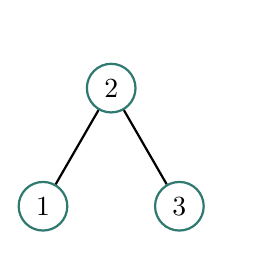
\begin{tikzpicture}
         \useasboundingbox (225:1.5) rectangle (45:2.5);

         \node (2) at (90:1) [circle, 
            draw=PineGreen!70!MidnightBlue, thick, fill=White] {2};
         \node (1) at (210:1) [circle, 
            draw=PineGreen!70!MidnightBlue, thick, fill=White] {1};
         \node (3) at (330:1) [circle, 
            draw=PineGreen!70!MidnightBlue, thick, fill=White] {3};
         \draw [thick] (1) -- (2);
         \draw [thick] (2) -- (3);
      \end{tikzpicture}
   \end{center}

\hOne
A \udefine{directed graph} (a.k.a a \udefine{digraph}) is a pair $(V, E)$ 
where $V$ is a set of vertices and $E$ is a set of ordered pairs 
of elements of $V$.
\begin{center}
   \hTwo
   For example: $G = (\{1, 2, 3\}, \{(1, 2), (2, 3)\})$

   \hThree
   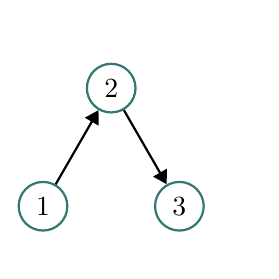
\begin{tikzpicture}
      \useasboundingbox (225:1.5) rectangle (45:2.5);

      \node (2) at (90:1) [circle, 
         draw=PineGreen!70!MidnightBlue, thick, fill=White] {2};
      \node (1) at (210:1) [circle, 
         draw=PineGreen!70!MidnightBlue, thick, fill=White] {1};
      \node (3) at (330:1) [circle, 
         draw=PineGreen!70!MidnightBlue, thick, fill=White] {3};
      \draw [thick, -Triangle] (1) -- (2);
      \draw [thick, -Triangle] (2) -- (3);
   \end{tikzpicture}
\end{center}

\hOne
A \udefine{multigraph} is a pair $(V, E)$ where $V$ is a set of vertices
and $E$ is a multiset of unordered pairs of elements of $V$.

\begin{center}
   \hTwo
   For example: $G = (\{1, 2, 3\}, \{\{1, 2\}, \{2, 3\}, \{2, 3\}\})$
   
   \hThree
   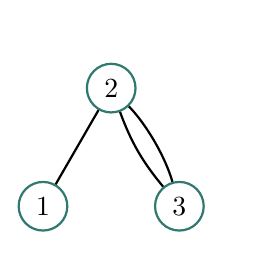
\begin{tikzpicture}
      \useasboundingbox (225:1.5) rectangle (45:2.5);

      \node (2) at (90:1) [circle, 
         draw=PineGreen!70!MidnightBlue, thick, fill=White] {2};
      \node (1) at (210:1) [circle, 
         draw=PineGreen!70!MidnightBlue, thick, fill=White] {1};
      \node (3) at (330:1) [circle, 
         draw=PineGreen!70!MidnightBlue, thick, fill=White] {3};
      \draw [thick] (1) -- (2);
      \draw [thick] (2) .. controls (50:.7) and (10:.7) .. (3);
      \draw [thick] (2) .. controls (50:.4) and (10:.4) .. (3);
   \end{tikzpicture}
\end{center}

\hOne
A \udefine{pseudograph} is like a graph and multigraph except that the
pairs in $E$ are multisets. 
\begin{myIndent}\begin{myIndent}\begin{myIndent}
\begin{myIndent}\begin{myIndent}
   \teachComment
   Essentially, an element $\{a, a\}$ can belong to $E$ in a 
   pseudograph. This type of edge is called a \udefine{loop}.
\end{myIndent}\end{myIndent}\end{myIndent}
\end{myIndent}\end{myIndent}

\begin{center}
   \hTwo
   For example: $G = (\{1, 2, 3\}, \{\{1, 2\}, \{2, 3\}, \{3, 3\}\})$
   
   \hThree
   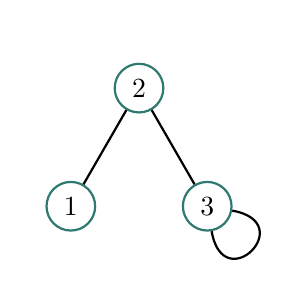
\begin{tikzpicture}
      \useasboundingbox (225:2) rectangle (45:2.5);

      \node (2) at (90:1) [circle, 
         draw=PineGreen!70!MidnightBlue, thick, fill=White] {2};
      \node (1) at (210:1) [circle, 
         draw=PineGreen!70!MidnightBlue, thick, fill=White] {1};
      \node (3) at (330:1) [circle, 
         draw=PineGreen!70!MidnightBlue, thick, fill=White] {3};
      \draw [thick] (1) -- (2);
      \draw [thick] (2) -- (3);
      \draw [thick] (3) to [out=350,in=280,looseness=6] (3);
   \end{tikzpicture}
\end{center}

\newpage
\hOne
If $G = (V, E)$ and $v \in V$, the \udefine{neighborhood} of $v$ is
$N_{G}(v)=\{w \in V \mid \{v, w\} \in E\}$. \bigbreak

The \udefine{degree} of $v$ is $d_{G}(v) = \lvert N_{G}(v) \rvert$.
Or in other words, $v$'s degree is equal to the number of edges 
connecting to $v$.

\mySepTwo[MidnightBlue]
\hTwo
\begin{myIndent}
   The \udefine{Handshaking lemma} states that for any graph $(V, E)$:
      {\fontsize{16}{15}\selectfont
      \[ \sum_{v \in V} d_{G}(v) = 2 \lvert E \rvert \]}
   
   \hThree
   \begin{myIndent}
      The reason for this is that each edge increments the degrees of
      exactly two vertices. So the above sum counts every edge twice.
      \hfill \bigbreak
   \end{myIndent}

   \hTwo
   \uuline{Lemma}: Every graph has an even number of vertices with odd
   degrees.

   \hThree
   \begin{myIndent}
      Proof: We can split the vertices of any graph into two categories:
      those with odd degrees, and those with even degrees.
      \hfill \bigbreak
      Now recall that an even number plus an even number always equals
      an even number, as does an odd number plus an odd number. However,
      an odd number plus an even numbers equals an odd number. Based on
      this fact, we can guarentee that the sum of even degrees in any
      graph is even. And since the sum of even degrees plus the sum of 
      odd\\ degrees must be even as it equals $2 \lvert E \rvert$ by
      the Handshaking lemma, we thus know that the sum of odd degrees 
      must be even. Hence, it must be the case that there are an even 
      number of vertices with odd degree because otherwise the sum of 
      their degrees won't be even.
      \hfill \bigbreak
   \end{myIndent}

   \hTwo
   A graph is called \udefine{$r$-regular} if all of its vertices have
   degree $r$.
   \hThree
   \begin{myIndent}
      Note that the number of edges in any $n$-vertex $r$-regular graph is
      $ \displaystyle{\frac{rn}{2}}$.
      \hfill \bigbreak
   \end{myIndent}
   
   \hTwo
   An $r$-dimensional \udefine{cube graph}, denoted as $\mathrm{Q}_{r}$,
   is a graph such that $V(\mathrm{Q}_{r})$, the set of vertices in 
   $\mathrm{Q}_{r}$, is equal to the set of binary strings of 
   length $r$; and $E(\mathrm{Q}_{r})$, the set of edges in 
   $\mathrm{Q}_{r}$, is equal to the set of pairs of binary strings
   which differ in only one position.

   \begin{center}
      \begin{tabular}{ c c }
         \hThree \fontsize{10}{10}\selectfont
         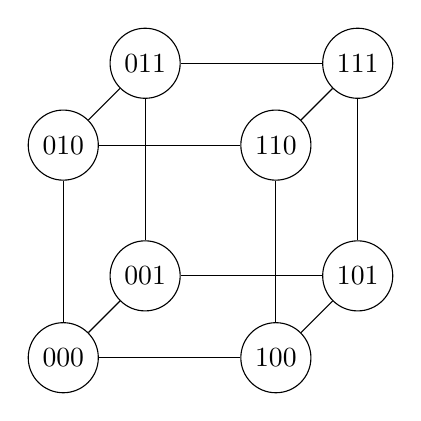
\begin{tikzpicture}[scale=0.9]
            \tikzstyle{myCir}=[circle,draw];
            \node[myCir] (000) at (0,0,0) {000};
            \node[myCir] (100) at (3,0,0) {100} edge (000);
            \node[myCir] (010) at (0,3,0) {010} edge (000);
            \node[myCir] (110) at (3,3,0) {110} edge (010) 
                                             edge (100);
            \node[myCir] (001) at (0,0,-3) {001} edge (000);
            \node[myCir] (101) at (3,0,-3) {101} edge (100) 
                                             edge (001);
            \node[myCir] (011) at (0,3,-3) {011} edge (010)   
                                             edge (001);
            \node[myCir] (111) at (3,3,-3) {111} edge (110) 
                                             edge (011) edge (101);
         \end{tikzpicture}
         & \hTwo
         ${\displaystyle \quad\quad\quad
         \begin{matrix}
            \lvert V(\mathrm{Q}_{r})\rvert = 2^{r} \\ \\
            \lvert E(\mathrm{Q}_{r})\rvert = \frac{2^{r}r}{2} = 
               2^{r-1}r \\ \\ \\ \\{\teachComment\text{
                  Note that } \mathrm{Q}_{r} \text{ is } r
                  \text{-regular.}}
         \end{matrix}}$
      \end{tabular}
   \end{center}
\end{myIndent}

\hOne
If $G=(V, E)$, then $H=(W, F)$ is a \udefine{subgraph} of $G$
if $W\subseteq V$ and $F\subseteq E$. \retTwo

If $W=V$, then $H$ is a \udefine{spanning} subgraph of $G$ (meaning 
that $H$ has the same vertices as $G$ but is lacking some of $G$'s 
edges) \retTwo

We define subtracting a set of vertices from a graph as follows:
\begin{myIndent} \hTwo
   For $G = (V, E)$ and $X \subset V$, we define...
      \begin{myIndent}\begin{myIndent}
         ${\displaystyle G - X = (V \setminus X, \{\{u, v\}\in E 
         \mid \{u, v\}\cap X = \emptyset\}) }$
      \end{myIndent}\end{myIndent}
\end{myIndent}
\retTwo

\hOne % I might not actually need this command here...
We define subtracting a set of edges from a graph as follows:
\begin{myIndent} \hTwo
   For $G = (V, E)$ and $L \subset E$, we define...
      \begin{myIndent}\begin{myIndent}\begin{myIndent}\begin{myIndent}
         ${\displaystyle G - L = (V, E \setminus L) }$
      \end{myIndent}\end{myIndent}\end{myIndent}\end{myIndent}
\end{myIndent}

\mySepTwo \hOne
\begin{myIndent}\begin{myIndent}\begin{myIndent}\begin{myIndent}
   Here are some basic classes of graphs: \retTwo
\end{myIndent}\end{myIndent}\end{myIndent}\end{myIndent}

\begin{itemize}
   \item \udefine{Complete graphs / cliques} are graphs where
      every possible edge is present. \hTwo 
      \begin{center}\begin{allowTableDashes}\begin{tabular}{ c;c;c;c }

         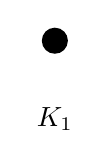
\begin{tikzpicture}
            \tikzstyle{myCir}=[circle, fill, radius=5pt];
            \node (name) at (270:1) {$K_{1}$};
            \node[myCir] (1) at (0:0) {};
         \end{tikzpicture} 
         
         & A & A & A
      \end{allowTableDashes}\end{tabular}\end{center}
\end{itemize}

\end{document}